\documentclass{scrartcl}

\usepackage[english]{babel}
\usepackage{lmodern}
\usepackage{color}
\usepackage[babel]{csquotes}
\usepackage{graphicx}
\usepackage{enumitem}
\usepackage{float}

\setcounter{secnumdepth}{0}

\bibliographystyle{unsrt}

\newcommand{\rulesep}{\unskip\ \vrule\ }

\title{Image classification with SVM}
\author{Andrea Portscher, Juan Pablo Stumpf, Philip Wille}

\begin{document}
\maketitle

\section{Introduction}
For this project we implemented an image classifier using three different feature extraction approaches: Scale-invariant feature transform (SIFT), Speeded up robust features (SURF) and Histogram of Gradients (HOG). First, we prepared an image dataset containing five different image classes, each comprising training and testing data. After extracting features using the above algorithms, we trained a Support-Vector Machine (SVM) and testetd, how well it was able to classify images.
\section{Approaches}
In the following section we will shortly explain the functionality of the feature extraction algorithms we applied to the dataset - namely SIFT, SURF and HOG.
In general, feature extraction algorithms work in three steps \cite{bay2006}:
\begin{enumerate}
  \item They select interest points at distinctive locations, such as corners.
  \item The neighbourhood of the interest points is represented by a feature vector.
  \item The descriptor vectors are matched between different images.
\end{enumerate}

\subsection{SIFT}
SIFT is a feature detection algorithm, which is invariant to similarity transformations and partially invariant to affine transformations. The algorithm consists of five steps:

\begin{enumerate}
    \item Scale space

        This step ensures the scale invariance, by blurring the image on different scales. This is similar a taking a photo at different distances. The blurring is done using the Gaussian convolution and on each step, the standard deviation is increased.

        \begin{figure}[H]
            \centering
            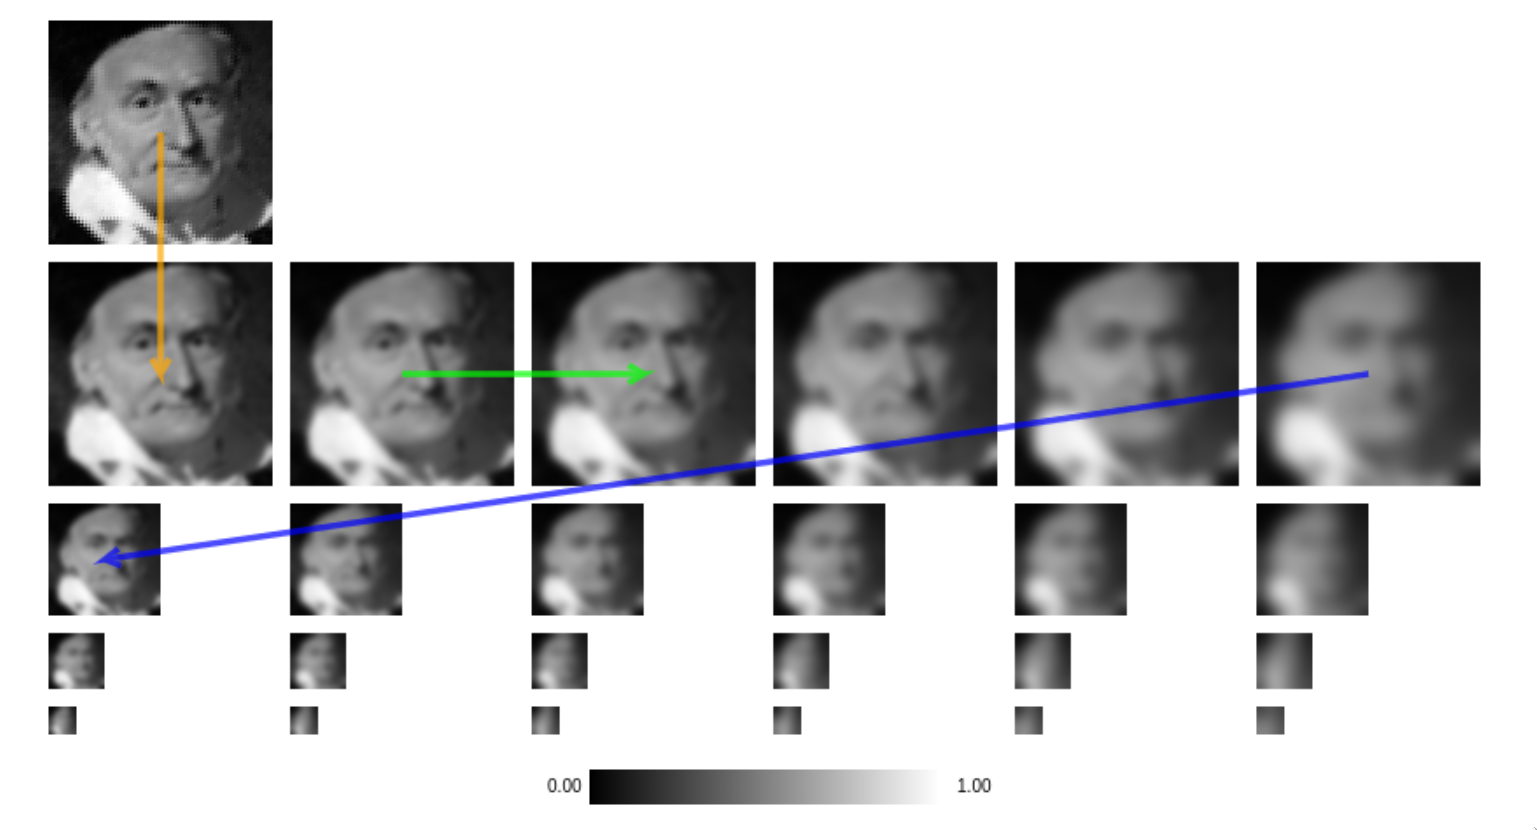
\includegraphics[width=0.6\linewidth]{img/sift1}
            \caption{Image blurred on different scales}%
            \label{fig:sift1}
        \end{figure}

        We can depict on the Figure~\ref{fig:sift1} how the image is once blurred (orange arrow), then the result is blurred again with a higher standard deviation (green arrow). The last image on the row is than downsampled, and the blurring begins again. This process is then done until the image is small enought.

    \item Extrema detection

        In this step, we look for pixel extremas by calculating the difference of Gaussians on the scale space. Then, the pixels are compared to their 26 neightbors, as we can see on Figure~\ref{fig:sift2}

        \begin{figure}[H]
            \centering
            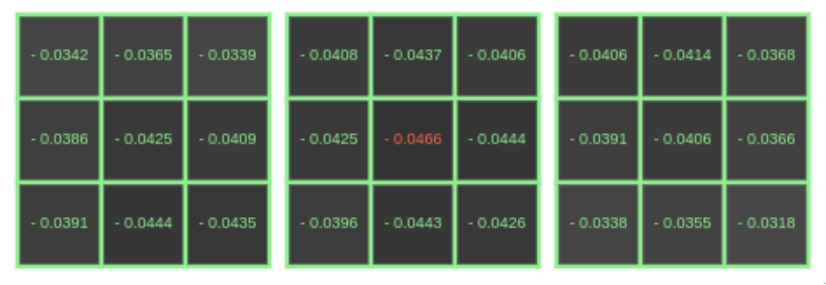
\includegraphics[width=0.5\linewidth]{img/sift2}
            \caption{Pixel neighborhood}%
            \label{fig:sift2}
        \end{figure}

    \item Keypoint localization

        Extremas lying on edges aren't good candidates, so they are removed. Also points with low contrast are discarded. On Figure~\ref{fig:sift3} we can appreciate the found extremas (left side) and the remaining extremas (right side).

        \begin{figure}[H]
            \centering
            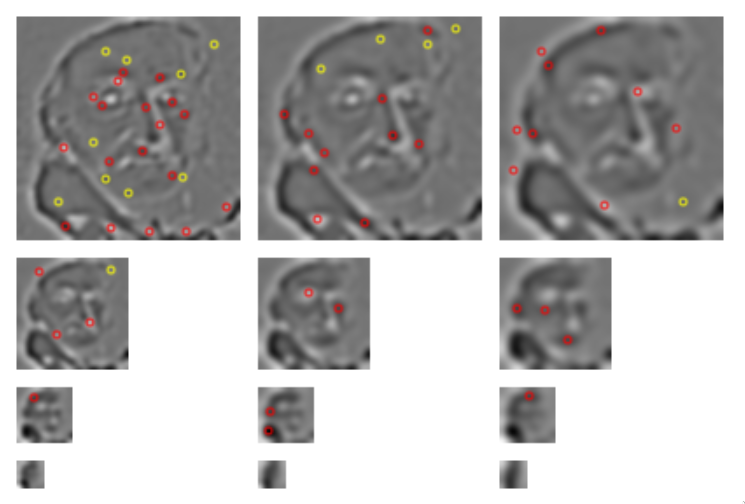
\includegraphics[width=0.4\linewidth]{img/sift3a}
            \rulesep
            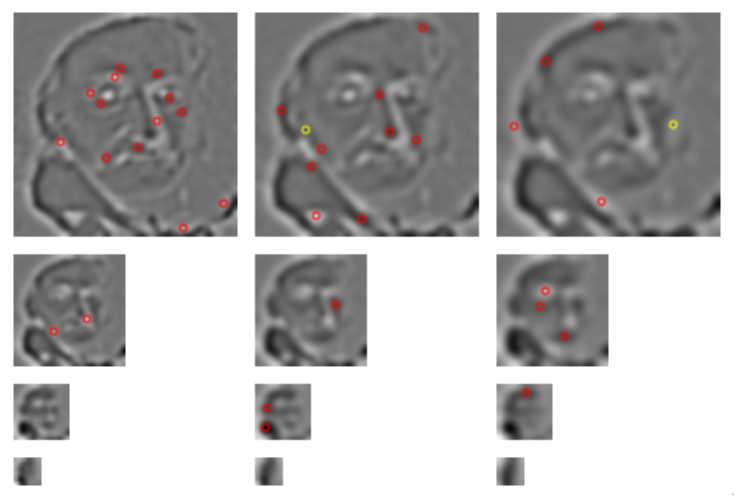
\includegraphics[width=0.4\linewidth]{img/sift3b}
            \caption{Calculated extremas}%
            \label{fig:sift3}
        \end{figure}

    \item Orientation assignment

        Now the gradient magnitude and orientation is calculated for each sample. A orientation histogram is created.

        \begin{figure}[H]
            \centering
            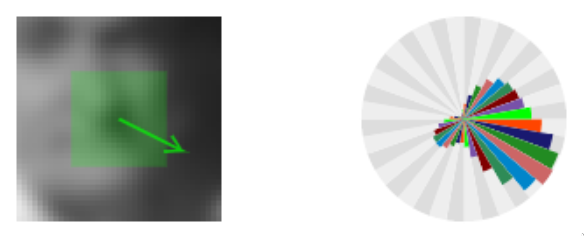
\includegraphics[width=0.4\linewidth]{img/sift4}
            \caption{Orientation histogram}%
            \label{fig:sift4}
        \end{figure}

        The left image on Figure~\ref{fig:sift4} depicts the dominant orientation, and the right image is the belonging histogram.

    \item Keypoint descriptor

        Finally, sixteen new histograms are calculated for each point near the center of the key point. The descriptor is composed of $4 \times 4 \times 8=128$ integers which is then our feature.

        \begin{figure}[H]
            \centering
            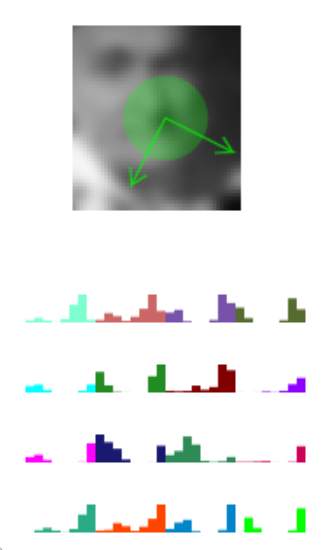
\includegraphics[width=0.2\linewidth]{img/sift5}
            \caption{Final descriptor}%
            \label{fig:sift5}
        \end{figure}
\end{enumerate}


\subsection{SURF}
SURF is based on similar properties as SIFT but is - as the name already takes away - faster and more robust. In the detection phase, SURF approximates the Laplacian of Gaussian with a box filter, and a convolution with a box filter can can easily be calculated with the help of integral images, and can be parallelized for different scales.
Another improvement is the use of the sign of the Laplacian for underlying interest points in the matching phase. Since it is already calculated during the detection phase, it comes at no additional cost, but speeds up the process by only comparing features if they have the same type of contrast\footnote{https://docs.opencv.org/3.4/df/dd2/tutorial\_py\_surf\_intro.html}.

Unlike SIFT, the SURF algorithm is currently still patented and can therefore only be used by including the \texttt{opencv\_contrib} package\footnote{https://github.com/opencv/opencv\_contrib} and allowing non-free algorithms.

\subsection{HOG}

The purpose of Histogram of Gradients (shortly HOG) is to count the occurrence of gradient orientations in a given image. The first time HOG was described by Robert K. McConnell of Wayland Research Inc. in a patent application in 1986 without using the term. It has become more famous when Navneet Dalal and Bill Triggs \cite{Hog_article} presented their work on HOG descriptors in their 2005 published paper.

\subsubsection{Functionality of HOG}

HOG decomposes an image into small squared cells, computes a histogram of oriented gradients in each cell, normalizes the result using a block-wise pattern, and return a descriptor for each cell. Stacking the cells into a squared image region can be used as an image window descriptor for object detection, for example by means of an SVM.

\section{Implementation}
\subsection{Data}
The image data we used stems from the Caltech-256 Image Set\footnote{http://www.vision.caltech.edu/Image\_Datasets/Caltech256/, accessed on the 22nd of December 2020}, which consists of 256 sets of images of a certain class. We randomly selected 5 of these, namely: cactus, dice, raccoon, spaghetti and sushi. The preaparation of the image data was comprised of the following steps, which we implemented in the file \texttt{utils.py}:
\begin{itemize}
  \item All images were resized to the same size, converted to grayscale and normalized (which removes noise from the image).
  \item All images are associated with a label (their image class).
  \item The images are split into a training set (80\% of images per class) and a testing set (20\% of images).
\end{itemize}

\subsection{Pipeline}
We use a pipeline\footnote{https://scikit-learn.org/stable/modules/generated/sklearn.pipeline.Pipeline.html} which sequentially applies a list of transforms and a final estimator.
In our case the transformers are the application of the respective feature extractor and finally the SVM.
The SIFT and SURF transformers are initialized in the same manner: After the features have been extracted, they are clustered.
In this step we used the MiniBatchKMeans clustering algorithm\footnote{https://scikit-learn.org/stable/modules/generated/sklearn.cluster.MiniBatchKMeans.html}. We used the Elbow Method to approximate the ideal size for K.
This approach works by simply calculating and plotting the distortions as a function of the number of clusters. Then the "elbow" of the graph - meaning the point in which the number of distortions starts to decrease too slowly to justify the additional cost of an increase in the number of clusters. The resulting graph for SIFT can be seen on the following figure. On this base we chose the value 500.
\begin{center}
  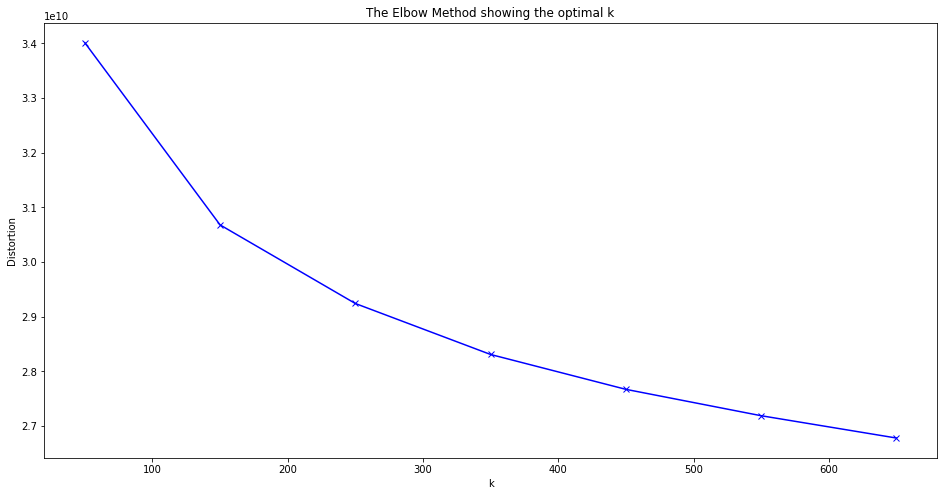
\includegraphics[scale=0.3]{img/kmeans-sift}
\end{center}
After having fitted the MiniBatchKMeans, the transformation begins and histograms are generated.
The next step in the pipeline is the training of the SVM. We chose the LinearSVC algorithm provided by the \texttt{sklearn} library\footnote{https://scikit-learn.org/stable/modules/generated/sklearn.svm.LinearSVC.html}.

For the HOG feature descriptor we only resize the incoming images to a size of 64 times 128 to be compliant with the paper of Navneet Dalal and Bill Triggs \cite{Hog_article}. The following steps are equal to these from SIFT or SURF.

\section{Discussion of Results}
In order to be able to evaluate our results we calculated metrics such as precision and recall and generated confusion matrices.
Furthermore, we used cross-validation. We checked the results for 2, 3, 4 and 5 image classes.
Naturally, all of the algorithms showed the best results with only 2 image classes and their reliability decreased with a rsing number of classes.

\bibliography{sources}

\end{document}
